\documentclass[a4]{article}
\usepackage[utf8]{inputenc}
\usepackage[french]{babel}
\usepackage{listings}
\usepackage{color}
\usepackage{graphicx}
\usepackage[T1]{fontenc}
\usepackage{pdfpages}
\usepackage{geometry}
\geometry{hmargin=2.5cm,vmargin=2.5cm}

\definecolor{mygreen}{rgb}{0,0.6,0}
\definecolor{mygray}{rgb}{0.5,0.5,0.5}
\definecolor{mymauve}{rgb}{0.58,0,0.82}

\lstset{
  backgroundcolor=\color{white},   % choose the background color; you must add \usepackage{color} or \usepackage{xcolor}
  basicstyle=\footnotesize,        % the size of the fonts that are used for the code
  breakatwhitespace=false,         % sets if automatic breaks should only happen at whitespace
  breaklines=true,                 % sets automatic line breaking
  captionpos=b,                    % sets the caption-position to bottom
  commentstyle=\color{mygreen},    % comment style
  deletekeywords={...},            % if you want to delete keywords from the given language
  escapeinside={\%*}{*)},          % if you want to add LaTeX within your code
  extendedchars=true,              % lets you use non-ASCII characters; for 8-bits encodings only, does not work with UTF-8
  frame=L,	                       % adds a frame around the code
  keepspaces=true,                 % keeps spaces in text, useful for keeping indentation of code (possibly needs columns=flexible)
  keywordstyle=\color{blue},       % keyword style
  language=C,                 	   % the language of the code
  otherkeywords={*,...},           % if you want to add more keywords to the set
  numbers=none,                    % where to put the line-numbers; possible values are (none, left, right)
  numbersep=5pt,                   % how far the line-numbers are from the code
  numberstyle=\tiny\color{mygray}, % the style that is used for the line-numbers
  rulecolor=\color{black},         % if not set, the frame-color may be changed on line-breaks within not-black text (e.g. comments (green here))
  showspaces=false,                % show spaces everywhere adding particular underscores; it overrides 'showstringspaces'
  showstringspaces=false,          % underline spaces within strings only
  showtabs=false,                  % show tabs within strings adding particular underscores
  stepnumber=2,                    % the step between two line-numbers. If it's 1, each line will be numbered
  stringstyle=\color{mymauve},     % string literal style
  tabsize=2,	                   % sets default tabsize to 2 spaces
  title=\lstname                   % show the filename of files included with \lstinputlisting; also try caption= instead of title
}
%gestion des caractères latins
\lstset{literate=
  {á}{{\'a}}1 {é}{{\'e}}1 {í}{{\'i}}1 {ó}{{\'o}}1 {ú}{{\'u}}1
  {Á}{{\'A}}1 {É}{{\'E}}1 {Í}{{\'I}}1 {Ó}{{\'O}}1 {Ú}{{\'U}}1
  {à}{{\`a}}1 {è}{{\`e}}1 {ì}{{\`i}}1 {ò}{{\`o}}1 {ù}{{\`u}}1
  {À}{{\`A}}1 {È}{{\'E}}1 {Ì}{{\`I}}1 {Ò}{{\`O}}1 {Ù}{{\`U}}1
  {ä}{{\"a}}1 {ë}{{\"e}}1 {ï}{{\"i}}1 {ö}{{\"o}}1 {ü}{{\"u}}1
  {Ä}{{\"A}}1 {Ë}{{\"E}}1 {Ï}{{\"I}}1 {Ö}{{\"O}}1 {Ü}{{\"U}}1
  {â}{{\^a}}1 {ê}{{\^e}}1 {î}{{\^i}}1 {ô}{{\^o}}1 {û}{{\^u}}1
  {Â}{{\^A}}1 {Ê}{{\^E}}1 {Î}{{\^I}}1 {Ô}{{\^O}}1 {Û}{{\^U}}1
  {œ}{{\oe}}1 {Œ}{{\OE}}1 {æ}{{\ae}}1 {Æ}{{\AE}}1 {ß}{{\ss}}1
  {ű}{{\H{u}}}1 {Ű}{{\H{U}}}1 {ő}{{\H{o}}}1 {Ő}{{\H{O}}}1
  {ç}{{\c c}}1 {Ç}{{\c C}}1 {ø}{{\o}}1 {å}{{\r a}}1 {Å}{{\r A}}1
  {€}{{\EUR}}1 {£}{{\pounds}}1
}
%definition d'un syle pour les documents text
\lstdefinestyle{txt}{
	frame=none,
	numbers=none,
	stringstyle=\color{black},
}

\begin{document}
	\title{\Huge{\textbf{Rapport Final}}}
	\author{Alabi Steve - Benyamna Younes - Capdenat Nicolas- \\
		Chouipe Thibaut - El Harti Zakaria - Lienhardt Florian \\ \\ \\
		Chef de projet : Benyamna Younes \\ \\ \\ 
		Sous la direction de Mme Kloul \\ \\ \\ \\
		Outil automatique de décryptage \\ \\ \\}
	\date{29 mai 2017}
		

	\begin{titlepage}
		\maketitle
		\vspace{20em}
		%\begin{center}
\includegraphics{logo_uvsq.jpg}\end{center}
	\end{titlepage}
	\section{Introduction}
Après avoir réalisé le cahier des charges, qui exprime les besoins/attentes du client ainsi que
les contraintes a respecter, et après avoir decrit comment les exigences fonctionnelles vont être implémentées(cahier des specifications)
, nous nous sommes donc lancés dans la réalisation du produit. \\ \\
Dcrypt est maintenant disponible et utilisable par le client. Un manuel d'utilisation
détaillé lui sera egalement fournit pour expliquer le fonctionnement de l'application.\\

Dans ce rapport, il s'agira de s'interesser tout d'abord à la logique/architecture de l'application et au choix du langage.
Enfin, nous pouvons nous pencher sur la partie technique du produit.
Pour cela, nous montrerons le fonctionnement de l'application à l'aide de tests, puis nous parlerons de l'organisation interne
 et pour finir nous verrons la comparaison du nombre de lignes de code réelles avec les estimations faites dans le cahier des charges.


	\section{Objectif de l'application}
	
	
	Le but du projet est donc de developper un logiciel pour automatiser le decryptage d'un texte.
	Le produit est réalisé afin de satisfaire le client, et pour se faire il doit répondre à toutes ses attentes.\\
	Ainsi, le client peut crypter ou decrypter un texte ou fichier et ce par methode de Substitution ou Vigenère.
	Mais aussi, il lui est possible d'effectuer independamment une analyse frequentielle sur un texte donné.
	
	

	\section{Architecture de l'application}
			\underline{Interface graphique :}     \hspace{5cm}  \underline{Cryptage Substitution :}\\
			- bouton cryptage            \hspace{5.5cm}       -créer une clé aleatoirement\\
			- bouton decryptage         \hspace{5cm}        -crypter le message\\
			- bouton substitution\\
			- bouton Vigenère           \hspace{5.2cm}       \underline{Cryptage Vigenère :}\\
			- affichage de texte(complet et partiel)  \hspace{2.2cm} -crypter le message\\
			- affichage pour la clé de substitution\\
			- bouton Francais(decryptage)   \hspace{3.5cm}     \underline{Decryptage Substitution :}\\
			- bouton Anglais(decryptage)    \hspace{3.5cm}     -decrypter le message\\
			- affichage pour l'analyse fréquentielle\\
			- charger un fichier texte       \hspace{4.2cm}  \underline{Analyse fréquentielle :}\\
			- sauvegarder un fichier texte     \hspace{3.8cm}  -analyse frequentielle sur texte donné\\
			- créer un nouveau fichier texte(resultats)\\
			- Demander clef de Vigenère\\
			
			\underline{Decryptage Vigenère :}\\
			-decrypter le message\\
			
			
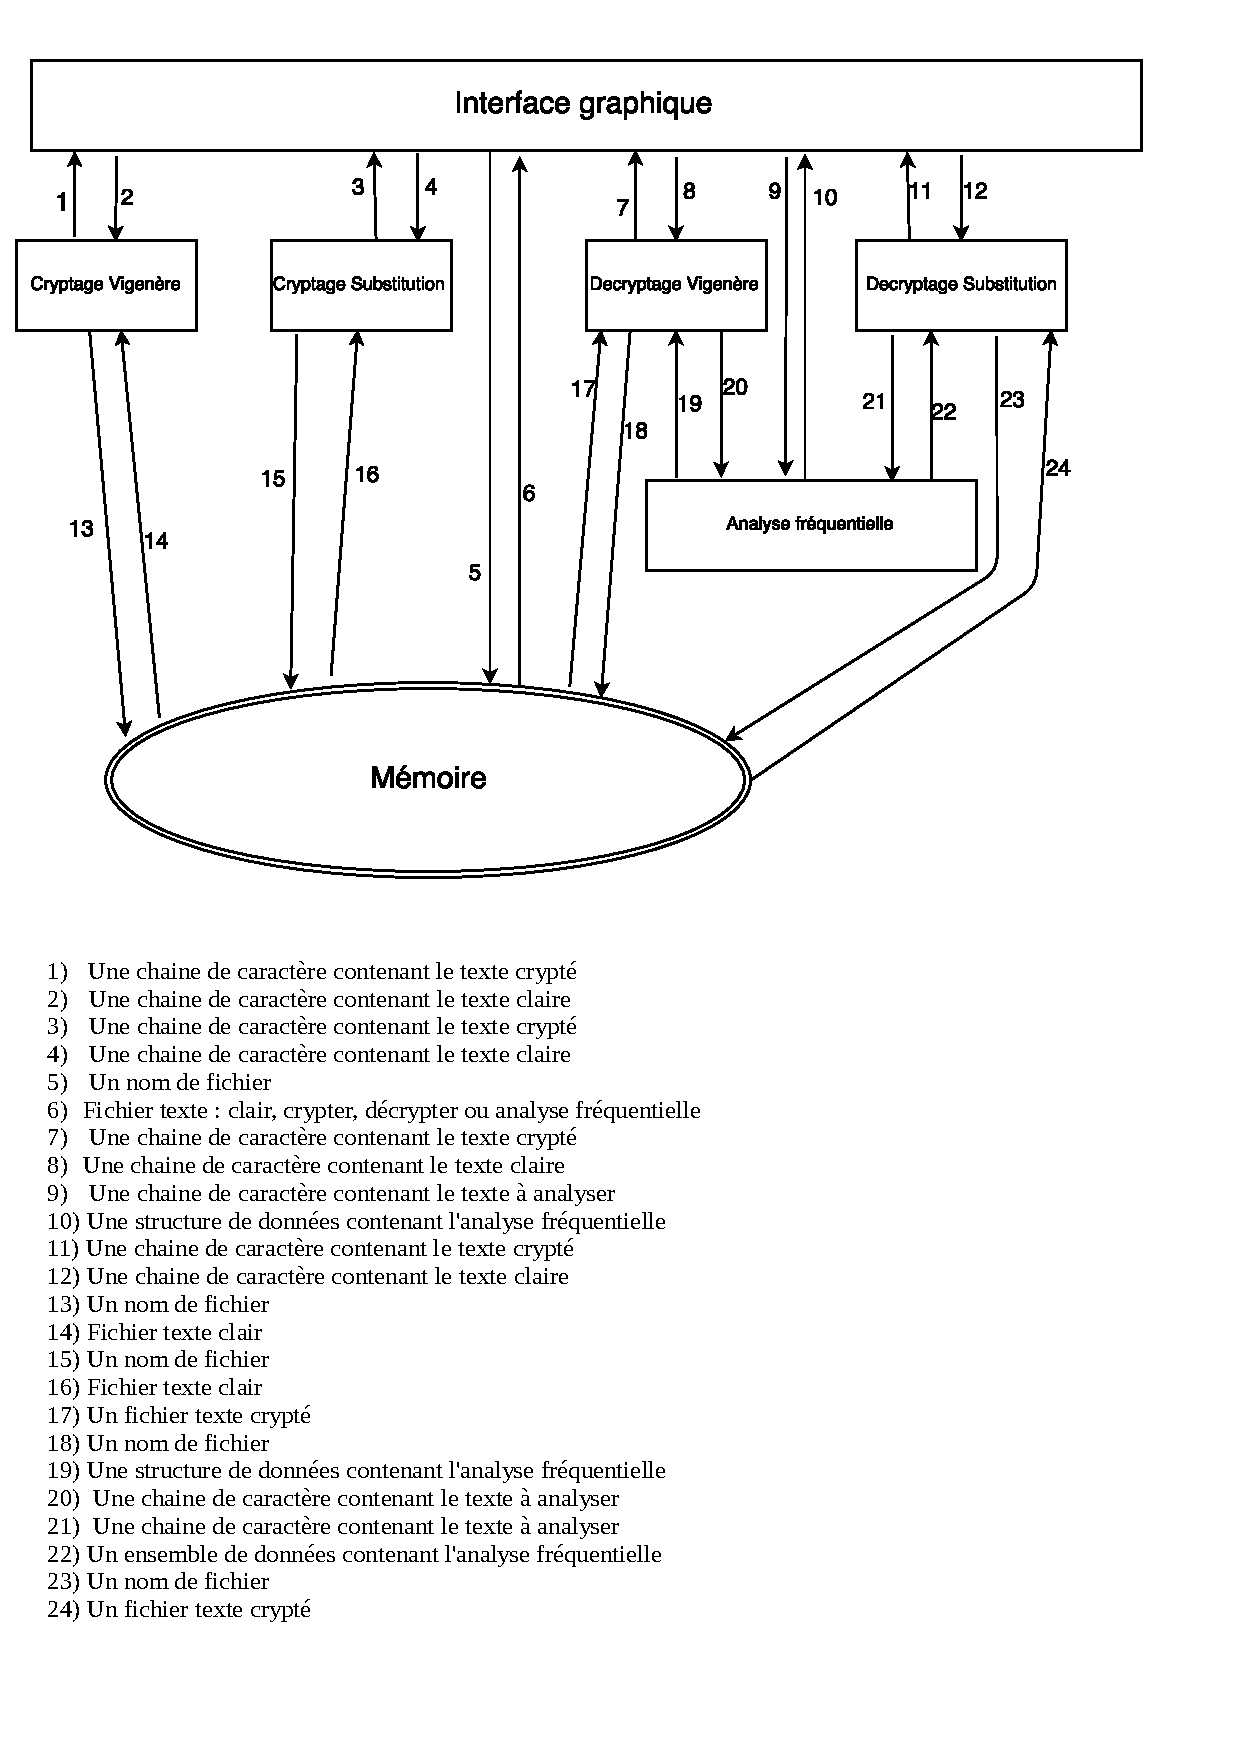
\includepdf[scale=0.9]{organ.pdf}


PRESENTATION DES MODULES DE L'ORGANIGRAMME.

	Notre organigramme se decompose en six modules:  un module d'interface graphique, un d'analyse 
	frequentielle,un de cryptage par substitution,un de decryptage par substitution,un de cryptage 
	par la methode de vigenere et un de decryptage par methode de vigenere. \\

	Le module d'interface graphique est le centre de notre programme dans le sens où il est le seul qui voit ses 
	fonctions appelées dans le main et qu'il interagit avec tous les autres modules en appellant leur fonctions principales.
	Son rôle principale est de metre à disposition de l'utilisateur une interface graphique 
	(composé de menus, de boites dialogue et de fenêtres). Ce module va egalement permettre à l'utilisateur de
	 paramétrer les options du logiciel, il pourra choisir la langue du texte (francais ou anglais) qu'il
	  pourra ensuite faire crypter, decrypter ou soummetre à une analyse fréquentielle. Pour se faire il aura
	   la possibilité de charger un fichier texte ou de taper un texte ainsi que d'enregistrer le texte crypté 
	   ou décrypté, la clef de cryptage en fonction de la methode utilisée ainsi qu'une analyse frequentielle. \\
	
	Le module d'analyse frequentielle va, comme son nom l'indique, effectuer une analyse frequentielle sur un texte donné.
	 Il va donc remplir une structure nommé structure ANALYSE en observant le nombre d'occurrences de chaque caractère du 
	 texte ainsi que les nombres d'occurrences des digrammes et trigrammes du texte.
	Ce module sera utilisé de trois manières differentes: il pourra être appelé pour l'analyse d'un texte donné,
	 pour permettre un décryptage par substitution ou pour permettre un décryptage par la methode de vigenere. \\

	Le module de cryptage par substitution va permettre de crypter un texte clair grace à la methode de la substitution
	 tout en creant une clef de sustitution aléatoire que l'utilisateur pourra sauvegarder via l'interface graphique. \\
	
	Le module de decryptage par substitution va permettre de decrypter un texte crypter par la methode de la substitution.
	 Ce module permettra d'obtenir un texte partiellement décrypté ainsi que la clef partielle de substitution. \\

	Le module de cryptage par la methode de vigenere va permettre de crypter un texte clair grace à la methode de vigenere
	 et d'une clef de cryptage rentrée par l'utilisateur. \\

	Le module de decryptage par la methode de vigenere va permettre de decrypter un texte crypté par la methode de vigenere. 
	Ce module permetra d'obtenir un texte décrypté ainsi que la clef utilisée lors du cryptage. \\ \\

	
PRESENTATION DES INTERACTIONS ENTRE LES DIFFERENTs MODULES DE L'ORGANIGRAMME ET DE LA MEMOIRE. \\

	L'interface graphique va intéragir avec la mémoire , elle va lui envoyer le nom de fichier entré par l'utilisateur 
	afin de recevoir le fichier texte en clair ou crypté correspondant. L'interface pourra également lui envoyer à la 
	memoire le nom de fichier ainsi que le texte crypté ou décrypté afin de l'enregistrer (fleche 5 et 6 sur le schema). \\

	L'interface graphique va intéragir avec le module de l'analyse frequentilelle, elle va lui envoyer une chaine de 
	caractère correspondant au texte à analyser entré par l'utilisateur. Le module d'analyse va lui renvoyer l'analyse 
	frequentielle sous la forme d'une structure analyse contenant le nombre d'occurrences de chaque lettre, des differents
	 digrammes et trigrammes que l'interface graphique pourra afficher (fleche 9 et 10 sur le schema). \\

	L'interface graphique va intéragir avec le module de cryptage par substitution, elle va lui envoyer une 
	chaine de caractères correspondant au texte en clair à crypter, et deux chaines de caractères vides. Le module
	 de cryptage par substitution va remplir les deux chaines de caractères vides, une avec le texte crypté obtenu
	  à partir du texte clair et l'autre avec la clef de substitution correspondante générée de façon aléatoire.
	   L'interface graphique pourra alors afficher ces deux chaines de caractères (fleche 3 et 4 sur le schema). \\

	L'interface graphique va intéragir avec le module de decryptage par substitution, elle va lui envoyer une 
	chaine de caractères corespondant au texte crypté à decrypter, et deux chaines de caractères vides. Le module 
	de decryptage par substitution va remplir les deux chaines de caractères vides, une avec le texte decrypté obtenu
	 à partir du texte crypté et l'autre avec la clef de substitution correspondante. L'interface graphique pourra 
	 alors afficher ces deux chaines de caractères (fleche 11 et 12 sur le schema). \\

	L'interface graphique va intéragir avec le module de cryptage par la methode de vigenere, elle va lui envoyer une
	 chaine de caractères corespondant au texte en clair à crypter,une chaine de caractères contenant la clef choisie par 
	 l'utilisateur et une chaine de caractères vides. Le module de cryptage par la methode de vigenere va remplir la chaine
	  de caractères vides avec le texte crypté obtenu à partir du texte clair et de la clef correspondante choisie par
	   l'utilisateur. L'interface graphique pourra alors afficher cette chaine de caractères (fleche 1 et 2 sur le schema). \\

	L'interface graphique va intéragir avec le module de decryptage par la methode de vigenere, elle va lui envoyer une 
	chaine de caractères correspondant au texte crypté à decrypter, et deux chaines de caractères vides. Le module de 
	decryptage par la methode de vigenere va remplir les deux chaines de caractères vides, une avec le texte decrypté 
	obtenu à partir du texte crypté et l'autre avec la clef de vigenere correspondante. L'interface graphique pourra 
	alors afficher ces deux chaines de caractères (fleche 7 et 8 sur le schema). \\

	Le module de l'analyse frequentilelle va intéragir avec le module de décryptage par substitution,
	 le module de décryptage par substitution va lui envoyer une chaine de caractères corespondant au texte 
	 crypté à analyser. Le module d'analyse va alors lui renvoyer l'analyse frequentielle de ce texte sous 
	 la forme d'une structure analyse contenant le nombre d'occurrences de chaque letrre, des differents digrammes 
	 et trigrammes que le module de décryptage utilisera pour décrypter le texte (fleche 15 et 16 sur le schema). \\

	Le module de l'analyse frequentilelle va intéragir avec le module de décryptage par la methode de vigenere, 
	le module de décryptage va envoyer à celui d'analyse une chaine de caractères correspondant au texte crypté à
	 analyser ainsi qu'un entier kasiski qui permettra de conjecturer la taille de la clef. Le module d'analyse va 
	 alors lui renvoyer l'analyse frequentielle de ce texte sous la forme d'une structure analyse contenant le nombre
	  d'occurrences de chaque lettre, des differents digrammes et trigrammes que le module de décryptage utilisera pour 
	  décrypter le texte (fleche 13 et 14 sur le schema). \\


	\section{Language choisi et explications}
	
	Le developpement de l'application s'est fait en langage C et les raisons étant les suivantes: \\
	
Nous avions besoin d'une application fonctionnelle et donc d'un langage procédurale. Le meilleur langage sur le marché
etant le C, le choix s'est logiquement porté sur ce dernier.\\ \\

Aussi, un argument de choix est celui de la portabilité. En effet, nous avions besoin d'une portabilité sur plusieurs
environnements et donc d'un besoin de standard ou norme. D'ou le langage C, car en effet il est possible d'utiliser
 le même programme sur tout autre système
 (autre hardware, autre système d'exploitation), simplement en le recompilant. \\ \\ \\



La bibliothèque graphique que nous avons décidée d'utiliser avec ce langage est GTK+ 
		parce qu'elle permet d'implémenter des boutons, des zones de texte, des menus ou encore du traitement de fichier.
		Elle nous semblait donc la plus adaptée au developement de notre application.
	\section{Partie technique}
	
	Tout d'abord, l'application fonctionne (compilation et execution) et
	l'ensemble des fonctionnnalités demandées par le client ont été réalisées.\\ 
	Les commandes pour compiler et executer sont les suivantes:\\
	-compilation:\\
	-execution:\\ \\
	
	
	Nous souhaitions avoir une application complète qui puisse tourner sur des ordinateurs 
de tout systeme d'exploitation et ce, sans pour autant qu’il ne
consomme trop de mémoire ou de temps processeur. \\ \\
	
	L'equipe de developpement a evidemment rencontré bon nombre de problèmes ou bugs. Voici pour chaque
	module une liste non exhaustive:
	\subsection{Interface graphique}
	-probleme du switch, remplacé par if..\\
	-
	\subsection{Analyse frequentielle}
	-probleme de segfault du a la gestion de la memoire: remplace "gchar* exemple" par "gchar exemple[10]"\\
	-
	\subsection{Decryptage vigenère}
 		Le decryptage fonctionne en deux parties :
 		
 		avec recherche automatique : test de Kasiski (marche 1 fois sur 3, taux de reussite plus important pour \\
 		des petites clés et peut eventuellement l'afficher en double (ex: clecle). 
 		*S'est effectué lors du premier clic gauche de l'utilisateur. \\
 		
 		Avec itération manuel pour trouver la taille de la clé car le test de Kasiski peut se tromper.
 		*Disponible après le premier clic gauche.
 		=> Permet d'augmenter considérablement le taux de réussite de Cryptanalyse d'un texte. \\
  		
 		Problèmes rencontrés avec Kasiski et l'hypothèse faite sur la taille de la clé. \\
  		 \\ \\
	
	\subsection{Decryptage substitution}
	-Nous avons sous-estimé le nombre de lignes attribués au module de cryptage de substitution,
	 ce problème couplé au nombreux changements à apporter aux structures, tableaux et differentes
	  variable à chaque fois que nous decryptions une lettre du texte crypté a vite rendu la fonction
	   prévue dans le cahier de spécification illisible et difficile à coriger et paramètrer. Ainsi 
	   pour permetrre une meilleur lecture du code nous avons divisé cette fonction en plusieur sous fonctions. \\ \\

	
		
		\subsection{Specifications}
		Des approximations et des erreurs de jugement sur le cahier des specifications ont conduit a certains changements ou problemes:\\
		-changement de la structure ( rajout de champs et de fonctions ainsi que la division de certaines fonctions en plusieurs
		 petites fonctions).\\
		-\\
		-\\ \\
		
		
		
		

		La decoupe technique des modules s'est faite en fonction des fonctionnalités.
		 Chacune de ces dernieres correspondant a un module.
		
		\subsection{Tests (unitaires)}
		L’exactitude des resultats de l'analyse etant tres importante pour les clients, nous avons predefinis des tests
unitaires pour chaque module(ou plutot les fonctions le composant). Ainsi, a chaque etape de la conception du logiciel
nous avons pu verifier que le calcul n’etait pas altere. \\ \\
Les tests permettent de voir comment le logiciel réagit lors de futurs améliorations ou d'une eventuelle maintenance. \\ 
 
Nous avons décidé d'utiliser Cunit qui est un systeme pour l'ecriture, l'administration et l'execution de tests unitaires
en langage C. Il fournit a son programmeur une fonctionnalité de test de base avec une variété d'interfaces utilisateur flexible.\\
Un "test"  CUnit est une fonction C ayant comme signature:\\
void\_test\_func()\\
Le corps de la fonction sera lui composé d'assertions Cunit.\\
Il y'aura création d'un registre et d'une suite de tests unitaires.\\
Nous noterons aussi la création automatique d'un Summary(récapitulatif) des tests.\\
remarque : besoin de l'option -lcunit a rajouter a la compilation des tests et d'inclure la bibliotheque avec un
\#include <CUnit/CUnit.h>.\\ \\ \\ 

  
Les resultats des tests unitaires sont les suivants:\\ \\ 
METTRE SCREEN TESTS "RUN" ICI \\ \\

		METTRE COMMANDE POUR COMPILER ET CELLE POUR EXECUTER TESTS
	\section{Organisation interne et affectation des taches}
	L'organisation de l'équipe est une chose importante pour le bon fonctionnement du
projet et le deroulement du codage, et est faite selon nos capacités et nos disponibilités.  \\ 
		 \begin{center}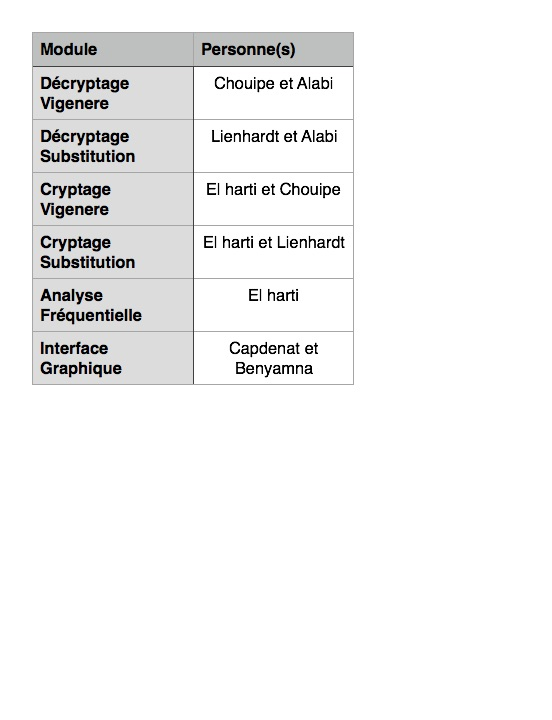
\includegraphics[scale=0.5]{tableau_tache_final.jpg}\end{center}
		 EXPLICATIONS SUR TABLEAU DES TACHES \\ 
		
		L'organisation etant bonne et la cohesion du groupe certaine, la repartition et la mise en place d'un planning 
		s'est faite naturellement et a été respectée.  \\
		La communication étant la clé d'un projet en groupe, nous avons préféré
		 nous reunir très regulierement et travailler tous ensemble et ce quel que soit l'etape du projet.
		\subsection{Planning de developpement}
		La phase de developpement constitue l’etape critique du projet, avec d’une part la decision de coder l’interface graphique
et d’autre part l’integration de tous les modules séparement. Lors de cette phase, les modules ont connu leurs dernieres evolutions ou plutot ajustements. \\
Avant de tester l’ensemble de l’application, nous avons dans un premier temps codé et
testé chaque fonction ou plutot module pour savoir si elles fonctionnaient séparément. \\
Nous les avons ensuite
réunies en les assemblant étapes par étapes pour construire l’application finale.  \\
--> en priorité : l'interface graphique consistait la base de l'application et devait donc être commencée et avancée tres rapidement \\
En evaluant les connaissances de chacun et en faisant un point regulierement sur nos taches respectives, cela a permis 
d'avancer efficacement dans la réalisation le projet.
	\section{comparaison lignes de code}
		\begin{center}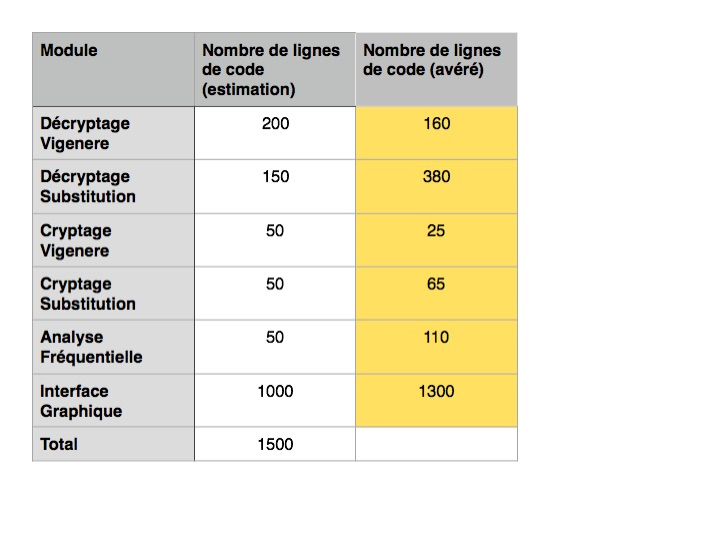
\includegraphics[scale=0.5]{preview.jpg}\end{center}
		Certains modules ont depassés le nombre de lignes estimées selon les raisons suivantes: \\
		-decryptage Vigenere : nombre de ligne trop juste au vu de certaines fonctions qui permettent de vérifier
		 nos résultats, par exemple la taille du mot clé. \\
		-cryptage substitution : il faut une fonction(tirage) qui va permettre qu'une lettre est toujours chiffrée
		 par une seule et meme lettre. \\
		-analyse frequentielle: fonction AnalyseFreq en plus qui est une tres legere variante de l'analyse des occurences de 
		chaque lettre faite deja dans AnalyseFrequentielle. Aussi, dans cette derniere, l'analyse des trigrammes fonctionne exactement
		comme celle des digrammes et donc on a repeté ces "autres" 40 lignes \\
		-interface graphique: pk??
		
	
	\section{Conclusion}
	-des choix a changer \\
	->au niveau des specifications et des fonctions \\ \\
	
	-critique du projet \\
	->Manque de reflexion ou d'approfondissement de certaines notions a des moments \\
	->?????? \\ \\
	
	
		
	-si a refaire, pareil?? \\
	->Le groupe serait le meme et la base du projet aussi. \\ \\ \\
	
	
	Finalement, nous avons une version "1.0" de l’application. La majorité des fonctionnalités
de base ont été implémentées et fonctionnent correctement mais il existe quelques
améliorations qui pourraient aboutir véritablement à une version "2.0" vraiment intéressante. \\
Quelques améliorations pourraient être ajoutées :
-Vigenere : ajout d'informations supplémentaire qui permettent d'aider/ameliorer le decryptage 
(exemple : on connait déja la taille de la clé).
-permettre a l'utilisateur de rentrer un type de texte (poeme, roman..) pour aider au decryptage \\
-plus de langues disponibles \\
-plus de cryptages/decryptages differents \\
=> Rajout d'un bouton "Recherche Intelligente" qui tente de trouver du premier coup la taille de clé.
-\\ \\ \\

	
	
Ce projet d'une durée d'un semestre(et plus precisement de 16 semaines) est une vrai expérience.
Cela a été enrichissant d'un point de vue personnel ou collectif:
il nous a apporté beaucoup, tant au
niveau technique qu’en terme de gestion de projet.  \\  \\
Nous connaissons maintenant l'importance du decoupage d'un projet en plusieurs etapes: cahier des charges, specifications,codage..
C'est un projet en "conditions d'entreprise" qui nous servira dans le futur.
C’est la première fois que nous travaillons en groupe a aussi nombreux sur un projet avec des caracteristiques bien définies. \\ \\
Nous sommes globalement satisfaits de ce que nous avons réalisé.
 Au niveau de la gestion du projet en équipe, nous avons réussi à bien nous répartir les
tâches afin de réaliser nos objectifs dans les temps et l'ambiance générale du groupe était très
bonne. \\ \\ \\





	
	
	
\end{document}
